
\documentclass[crop,dvipsnames,tikz]{standalone}

\usetikzlibrary{calc}

\definecolor{darkorchid}{rgb}{0.6, 0.2, 0.8}

\begin{document}
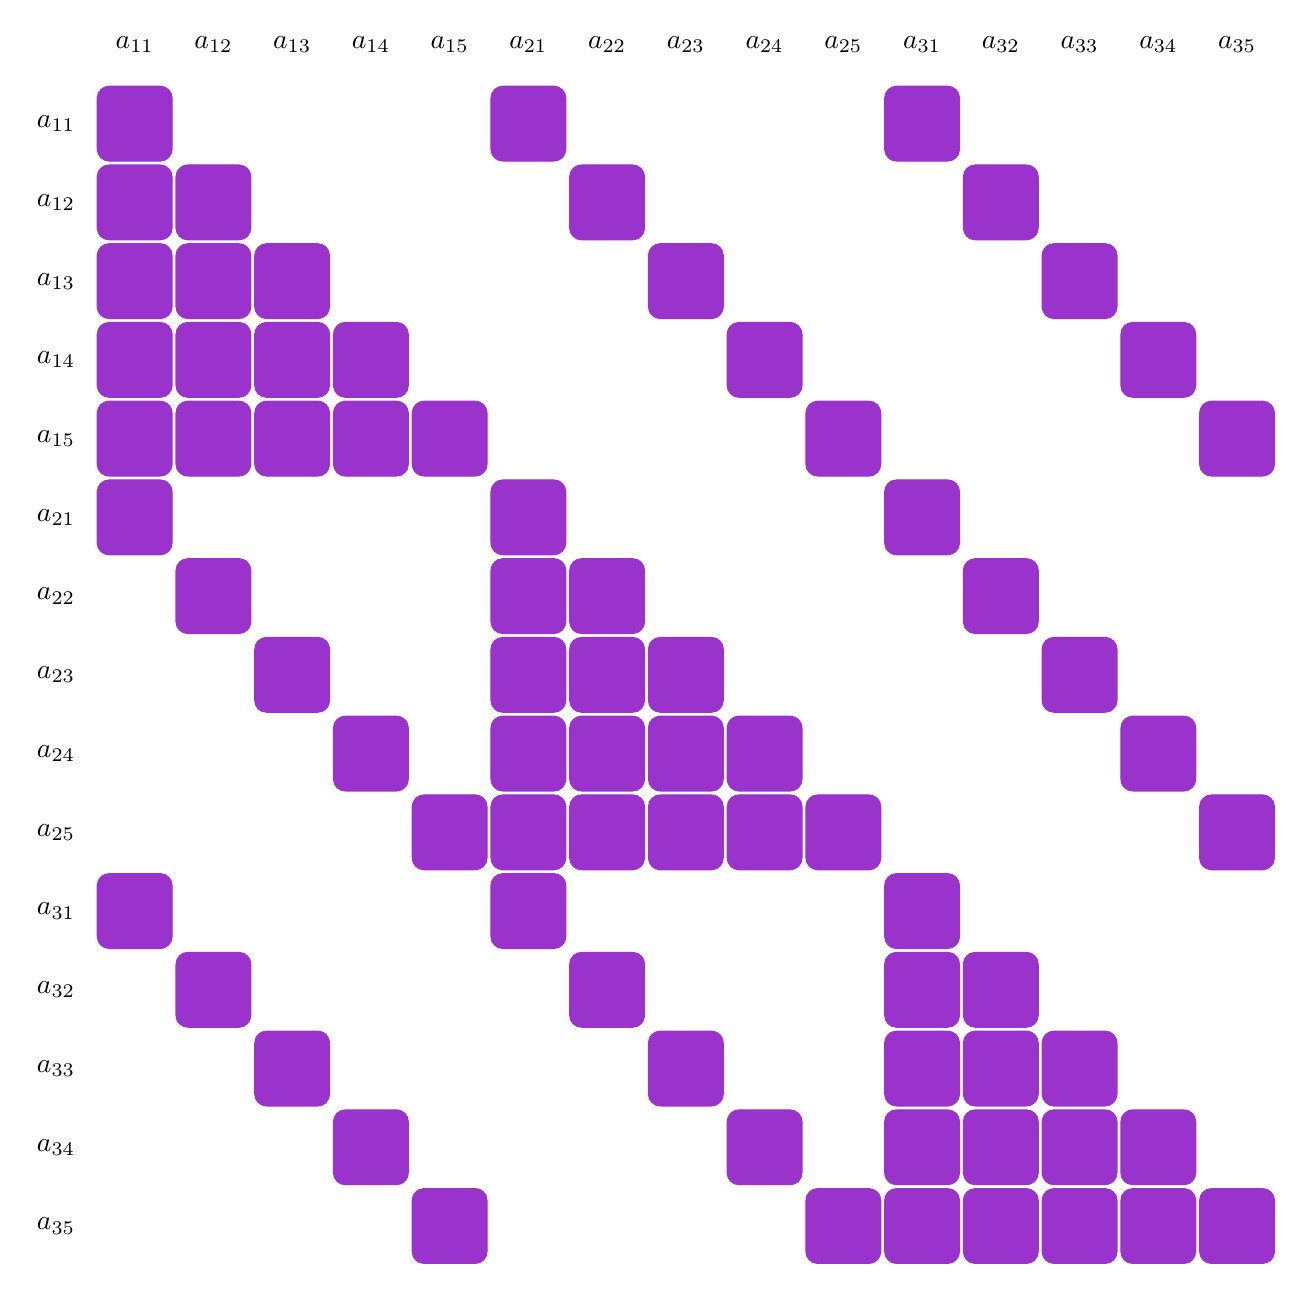
\begin{tikzpicture}
    \foreach \a in {1,...,3} {
        %\foreach \i in {0,...,5} {
        %    \node at (\i+0.5, 6.5) {$a_{\a\i}$};
            \foreach \j in {1,...,5} {
                \node at (\a*5+\j-5,16) {$a_{\a\j}$};
                \node at (0,16-\a*5-\j+5) {$a_{\a\j}$};
                \foreach \aa in {1,...,3} {
                    \foreach \jj in {1,...,5} {
                     
                        %% when j < jj and a == aa
                        \ifnum \j<\jj \ifnum \a=\aa
                            \node[fill=darkorchid, draw=darkorchid, minimum size=.95cm, inner sep=0pt, outer sep=0pt, rounded corners=1ex] at (\a*5+\j-5,16-\aa*5-\jj+5) {};
                        \fi\fi
                        \if \j\jj
                            \node[fill=darkorchid, draw=darkorchid, minimum size=.95cm, inner sep=0pt, outer sep=0pt, rounded corners=1ex] at (\a*5+\j-5,16-\aa*5-\jj+5) {};
                        \fi
                        
                    }
                }
            }
        %}
    }
\end{tikzpicture}
\end{document}

